\documentclass{../grid-link-report}
\SetClassAssetsDir{../class-assets}

\newcommand{\projectassetsdir}{../project-assets}

\project{Heywood BESS}
\client{ATMOS}
\title{Voltage Control Strategy}
\docnumber{HEYWOODBESS-GR-RPT-003}
\issueddate{30 July 2025}
\revision{1-1-0}
\revisionhistorycsvpath{report-assets/revision-history.csv}
\clientlogopath{\projectassetsdir/client-logo.jpg}

\usepackage{listings}
\usepackage{tabto}
\usepackage[justification=centering]{caption}%
\usepackage{pgfplotstable} % For reading and displaying tables from CSV files
\usepackage{booktabs}      % For better-looking tables

\begin{document}
	% Draft commands
	%\adddraftstamp
	
	\frontmatter
	\maketitle
	
	\makedisclaimer
	\clearpage
	\tableofcontents
	\makerevisionhistorypage
	%\makeaboutgridlink
	
	\mainmatter
	
	\chapter{Introduction}
	
	\section{Project overview}
	The \ac{Heywood BESS} is a $\pm~285MW/1140MWh$ Battery Energy Storage Project, located 5 km from the town of Heywood and 300 km west of Melbourne in Victoria. As part of this project, the new  275kV underground cable will be constructed between \ac{Heywood BESS} site and existing 275 kV switchyard.

\ac{Heywood BESS} will include 92 * SMA Sunny Central 4.6 MVA (SCS 4600 UP-S) inverters which will be connected to two 275/33/33 kV, 160MVA transformers through the 33kV reticulation system. Each inverter will have a dedicated 33/0.69kV, 4.6 MVA step up transformer.

\ac{Heywood BESS} will operate in voltage droop control mode by default, controlling the 275kV connection point with a 4\% droop on a 112.575 MVAr base.

The proposed maximum capacity of \ac{Heywood BESS} at the connection point is $\pm$ 285 MW at ambient air temperatures up to 50°C. 

{
	\thicktablelines
	\begin{longtable}{|C{5cm}|C{10cm}|} 
		\caption{Connection Overview}
		\label{tab:connection-overview}
		\\	
		\toprule
		
		\rowcolor{tableheaderblue}
		\bfseries \color{white}Connection Overview & \bfseries \color{white}Description\\
		\endhead
		\bottomrule \endfoot
		\csvreader[
		separator=semicolon,
		late after line=\\\hline,
		late after last line=,
		before reading={\catcode`\#=12},
		after reading={\catcode`\#=6}]%
		{report-assets/connection_overview.csv}{1=\CSVOverview,2=\CSVDescription}{\CSVOverview & \CSVDescription}
		\\\hline
	\end{longtable}
}


	

	\chapter{Voltage control strategy}
	
	\section{Plant layout}
	
	The PSCAD model is an aggregated representation of the BESS, and is used to demonstrate the proposed structure of the plant for purposes of the \ac{VCS}. Four lumped inverter models, including unit transformers from 0.69/33 kV are connected to the MV sides of two  275/33/33 kV three-winding grid transformers via lumped impedances representing the reticulation network. This model consists of:
	
	\begin{itemize}
		\item The grid element, which provides facilities to configure the grid SCR and X/R, apply faults and other disturbances.
		\item The point of connection.
		\item 1 x 275 kV underground cable between substation and \ac{POC}.		
		\item Two main three-winding 275/33/33 kV transformers with \ac{OLTC}.
		\item Four aggregated MV reticulation representing the lumped impedance of 33kV feeders (modelled as X,R,B quantities)	
		\item Four aggregated MV reticulation representing the lumped impedance of 33kV transformers to 33kV switch room (modelled as X,R,B quantities)
		\item Four two-winding MV 33/0.69 kV inverter transformer and current multiplier to represent all ninety-two (92) inverters.
		\item Four lumped SCS 4600 UP-S inverter models. 
	\end{itemize}
	
	The PSCAD single line diagram of the single machine infinite bus model for the BESS is shown in the below Figure \ref{fig:pscad-model-sld}.
	
	\begin{figure}[H]
		\centering
		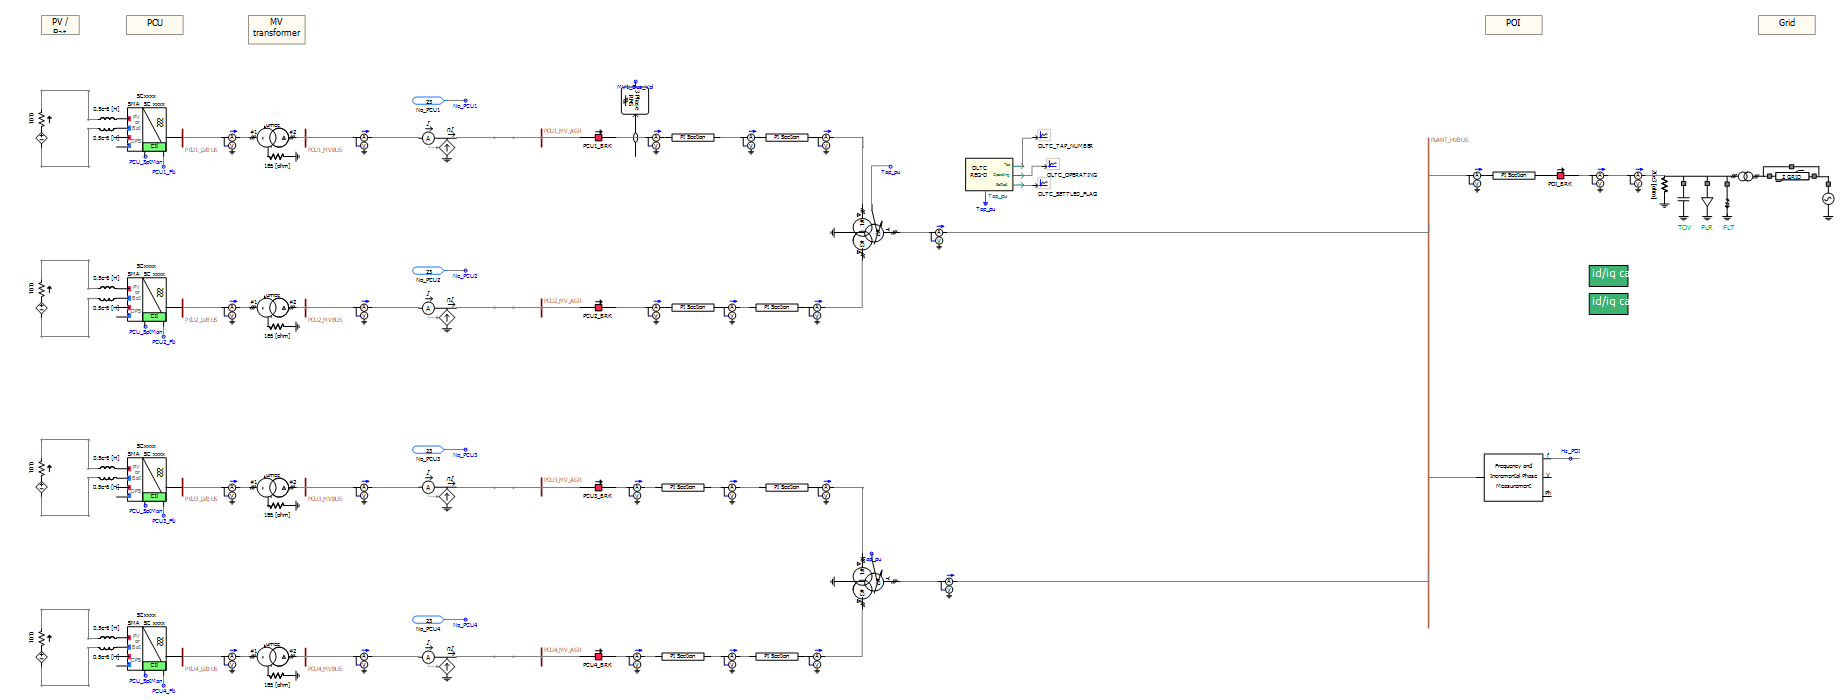
\includegraphics[width=0.9\textwidth]{report-assets/images/pscad-model-screenshot.png}
		\caption{PSCAD SMIB model SLD}
		\label{fig:pscad-model-sld}
	\end{figure}
	
	
	\section{Control scheme configuration}
	
	\subsection{Power plant controller}
	
	\subsubsection{Reactive power control modes}
	
	The \ac{PPC} acts as an outer loop controller for the plant, sending set-point commands for active and reactive power to converters to control flows at the 275 kV point of connection, regardless of control strategy selected. The Fluence PPC is capable of operating in multiple modes to regulate reactive power flow.
	
	\begin{itemize}
		\item Power factor control
		\item Remote reactive power control
		\item Voltage droop control
	\end{itemize}
	
	Under normal operation, it is expected that the PPC will be set to mode 5 - voltage droop control, to target a voltage setpoint of 1.06 p.u. on a 4\% droop, with limits at ±112.575 MVAr. The PPC is capable of controlling the response of the plant under normal operating conditions, but if voltage at the point of connection is outside the 0.85 to 1.15 p.u. range the PPC will freeze the value of the setpoint that it is sending, which is indicated by a PPC freeze flag signal (FRT signal). Under these circumstances, plant converters will control voltage at their own terminals independently via droop control, or will enter FRT mode. These modes of operation are explained in Section \ref{sec:inverter-level-control}.
	
	
	\subsubsection{Voltage droop control}
	
	The PPC is set to voltage droop control by default, with a droop of 4\% specified for the plant. The PPC targets a setpoint (expected to be 1.06 p.u. in line with the current normal operating voltage at the Heywood 275 kV connection point) to control voltage under a droop characteristic at the generator point of connection. No deadband has been specified for voltage droop control at the point of connection (POC).
	
	
	The PPC droop characteristic is shown in Figure \ref{fig:vdroop-char}.
	
	\[
	\text{Droop} =  \left[ \frac{\text{p.u.}}{\text{p.u.}} \right] = \frac{(U - U_{\text{set}})/U_n}{(Q - Q_{\text{set}})/Q_n} = \frac{U - U_{\text{set}}}{Q - Q_{\text{set}}} \cdot \frac{Q_n}{U_n}
	\]
	(with Qn = 112.575 MVAr)
	
	\begin{figure}[H]
		\centering
		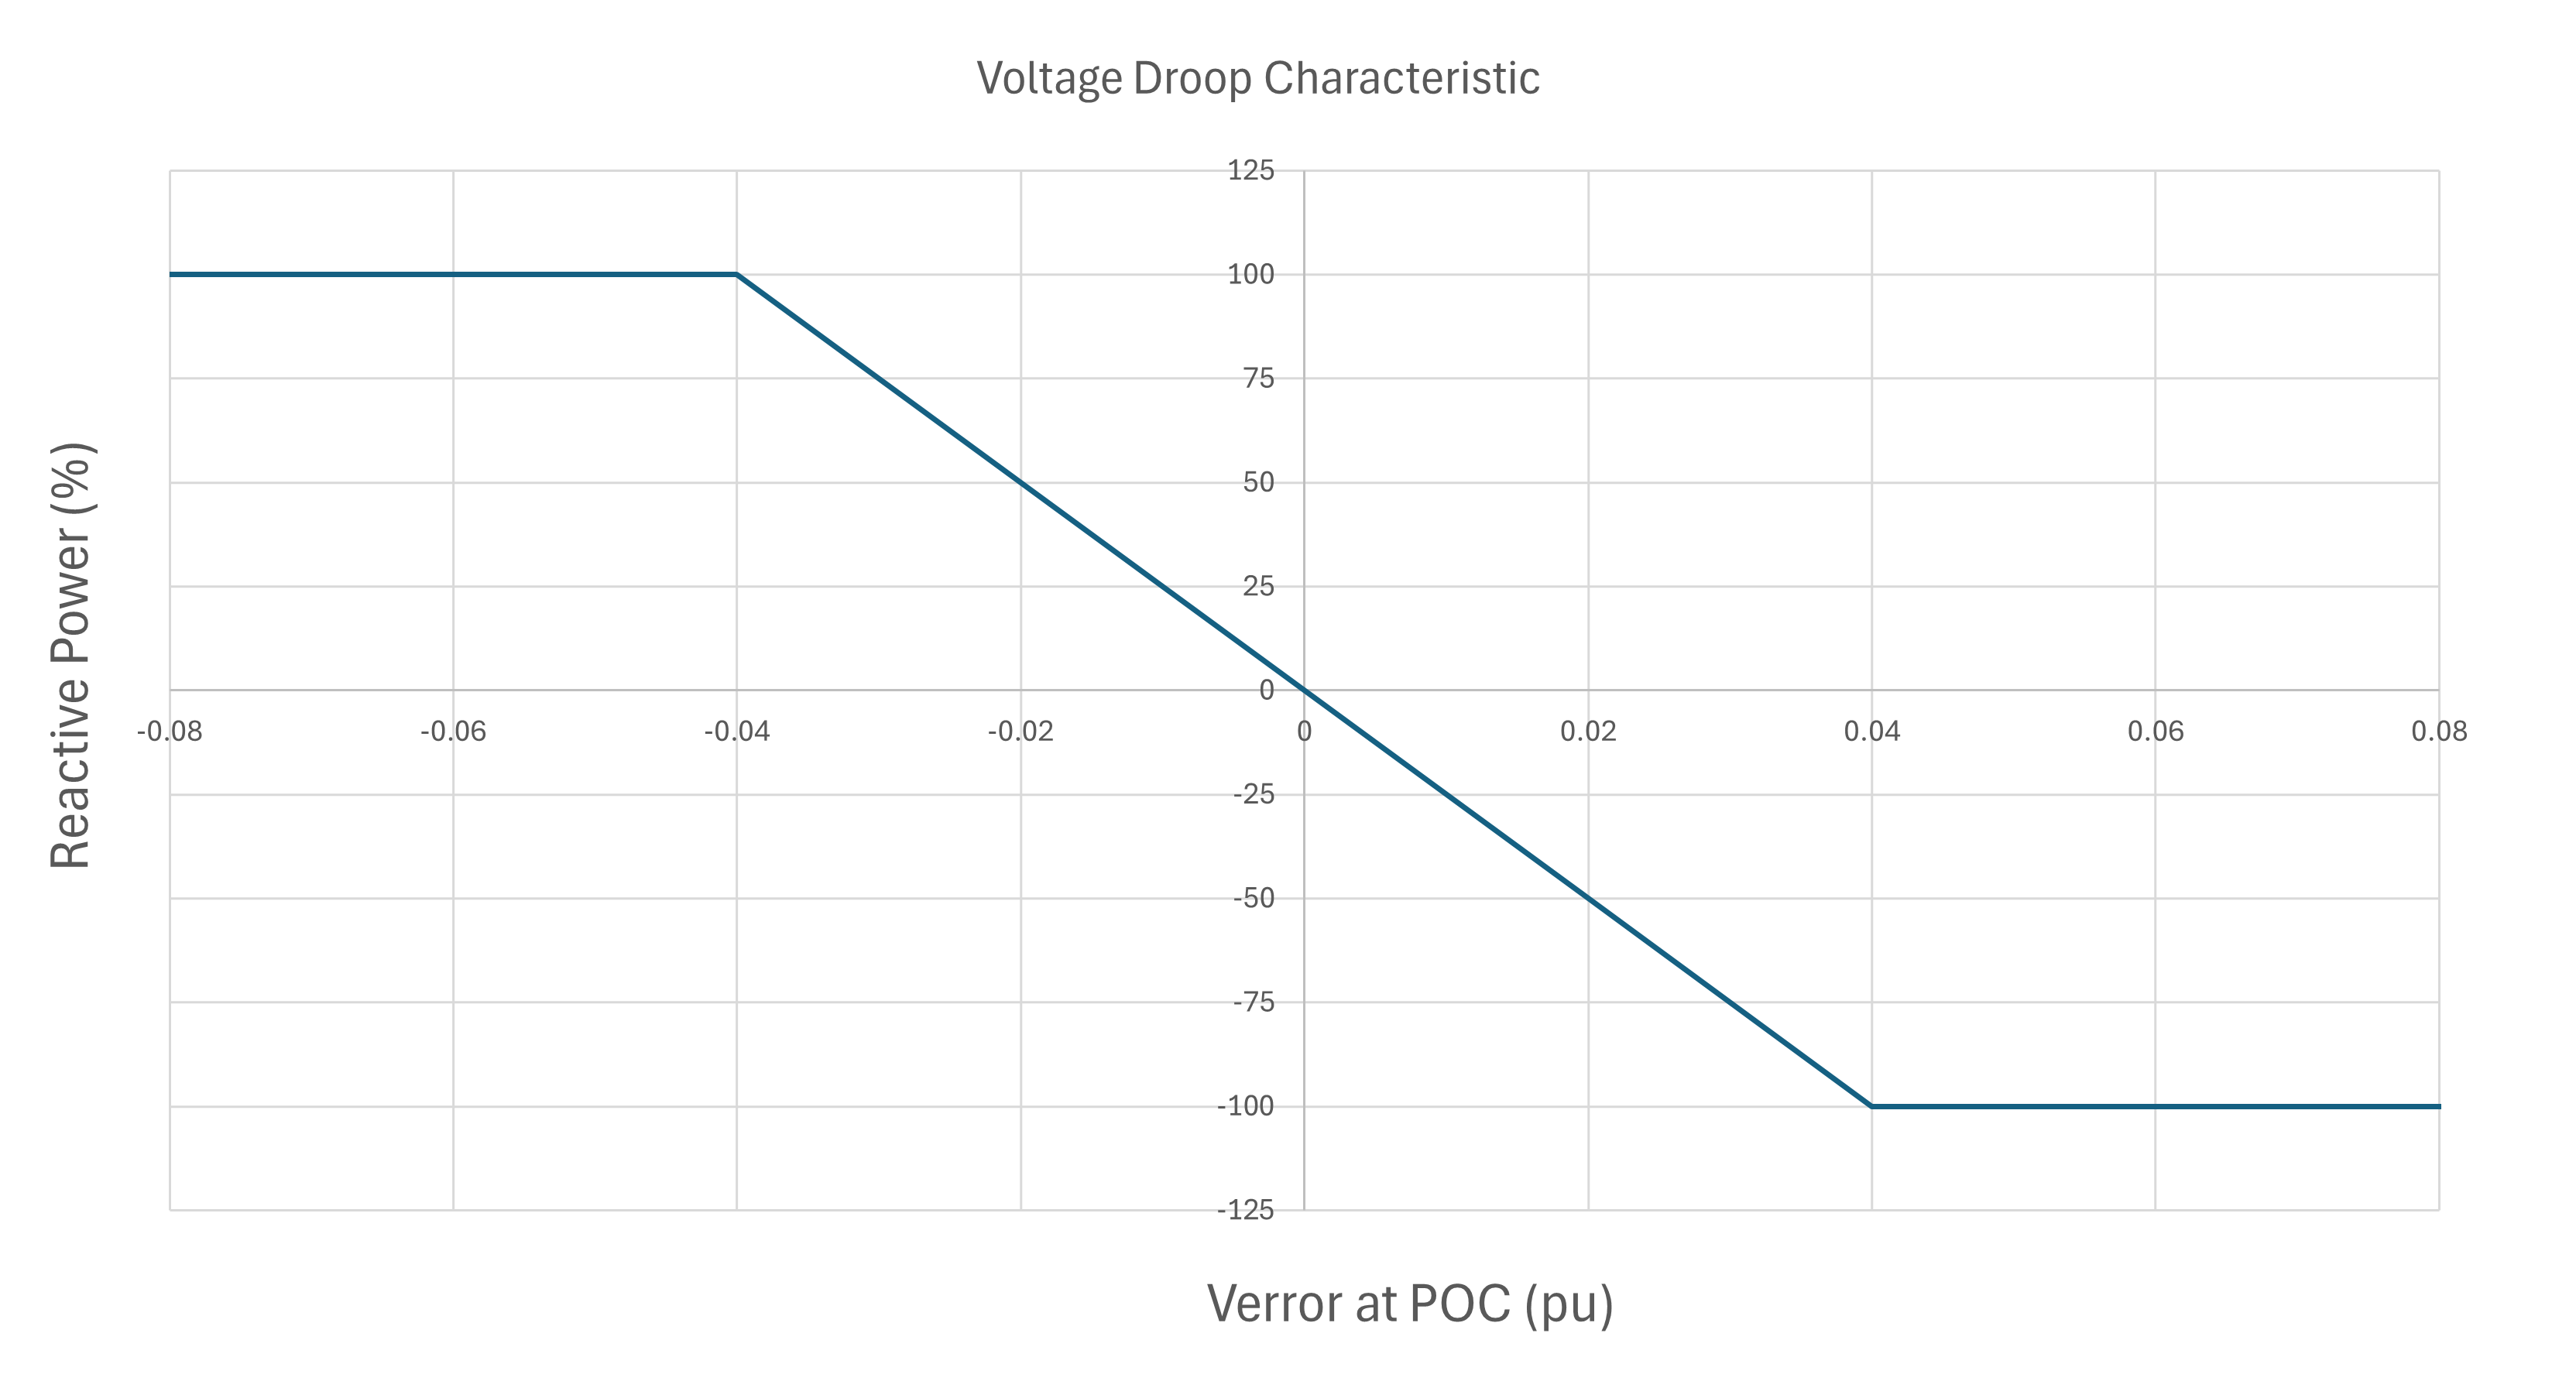
\includegraphics[width=0.9\textwidth]{report-assets/images/vdroop-char.png}
		\caption{Voltage droop characteristic}
		\label{fig:vdroop-char}
	\end{figure}
	
	The values for $\pm 100 \%$ are shown in table below.
	\dansquicktable{|C{5cm}|C{4cm}|C{4cm}|C{4cm}|}
	{Voltage droop characteristic tabulated}
	{v-droop-char}
	{\bfseries \color{white} & \bfseries \color{white}Normal voltage (pu) & \bfseries \color{white}Voltage at POC (pu)) & \bfseries \color{white}Reactive Power (MVAr)}
	{report-assets/v-droop-char-new.csv}
	
	The block diagram for the voltage droop control mode is shown in Figure \ref{fig:vdroop-block-diagram}.
	
	\begin{figure}[H]
		\centering
		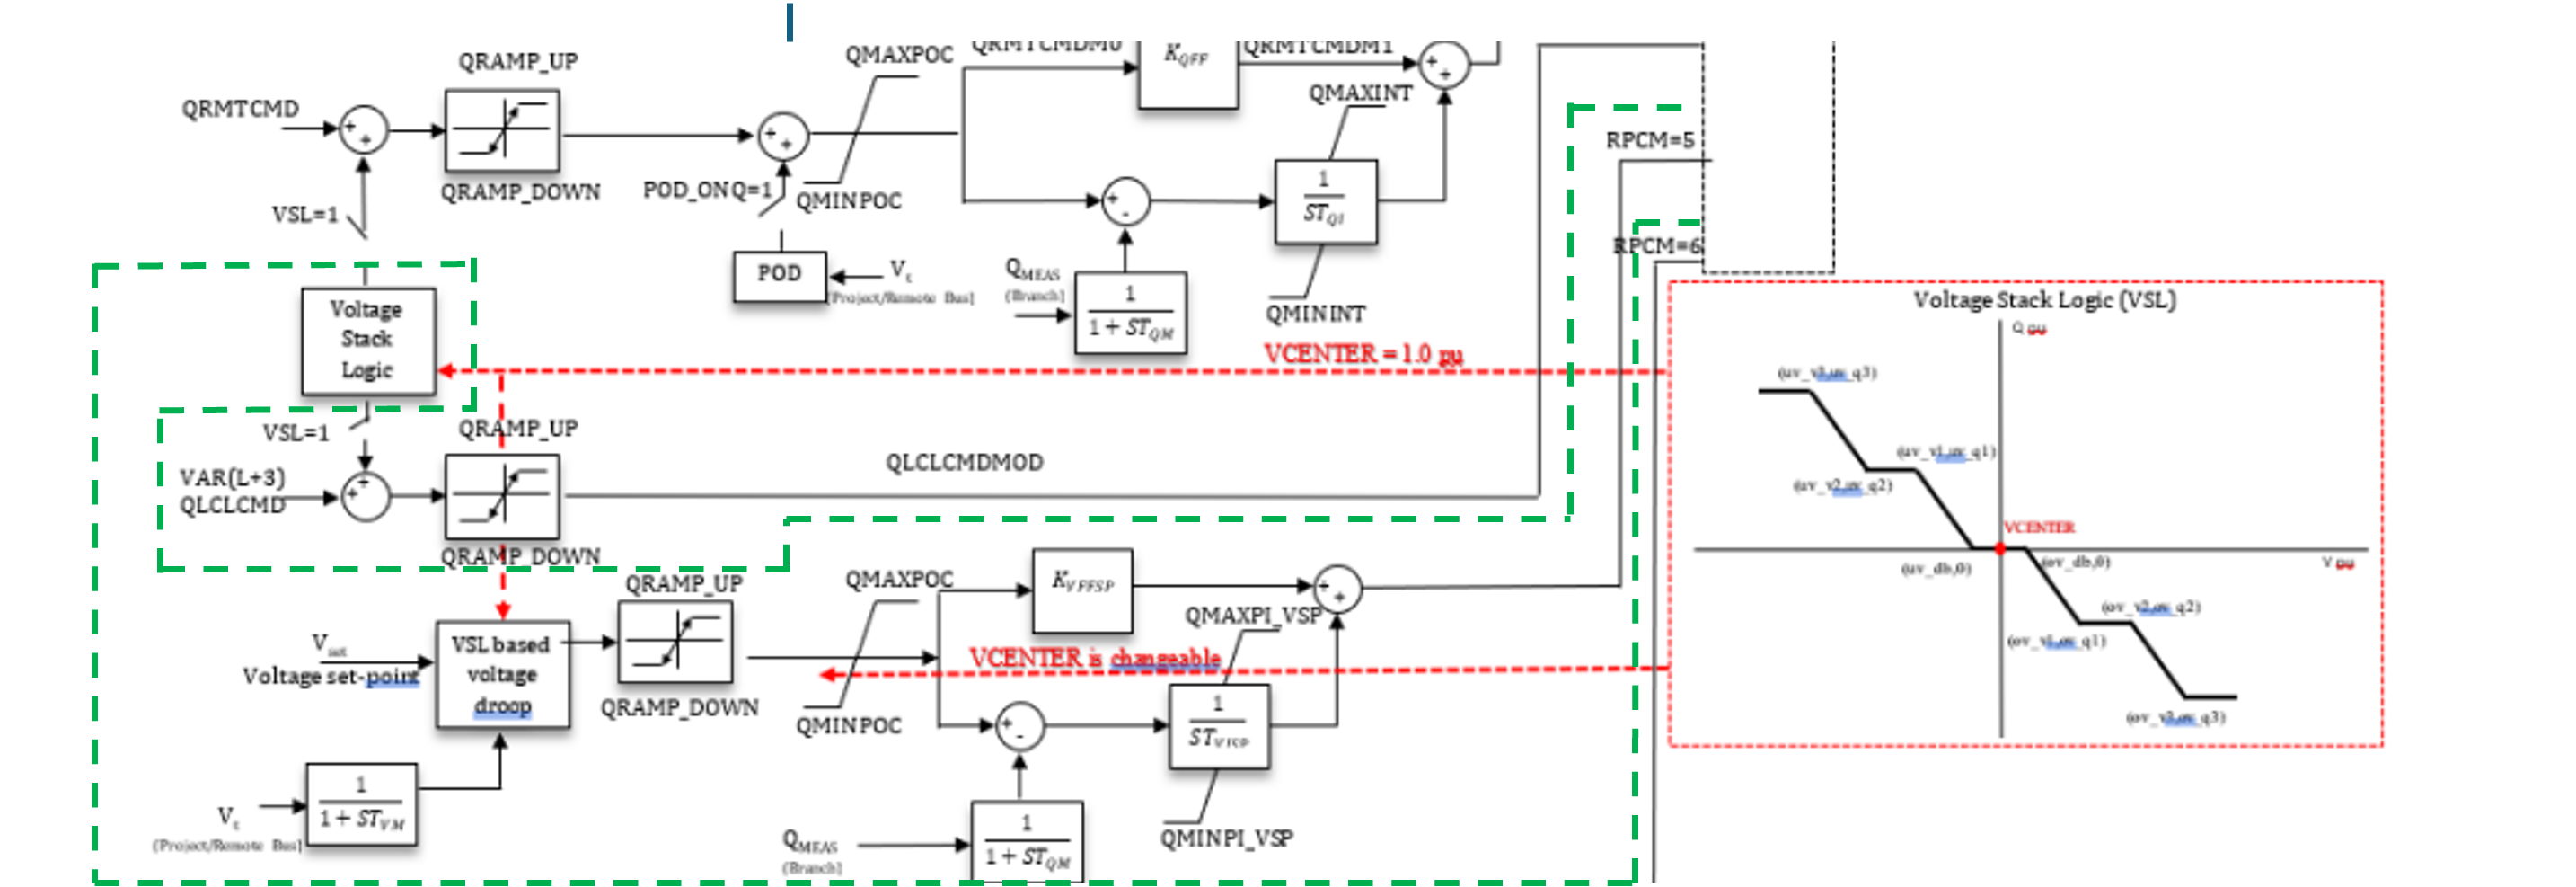
\includegraphics[width=0.6\textwidth]{report-assets/images/vdroop-mode-block-diagram.png}
		\caption{Voltage droop control block diagram}
		\label{fig:vdroop-block-diagram}
	\end{figure}
	
	\subsubsection{Remote reactive power control}
	
	Remote reactive power control is available in the PPC. This allows the PPC to target a constant reactive power setpoint at the point of connection, within the limits of the plant rating. The block diagram for the remote reactive power control mode is shown in Figure \ref{fig:q-block-diagram}.
	
	\begin{figure}[H]
		\centering
		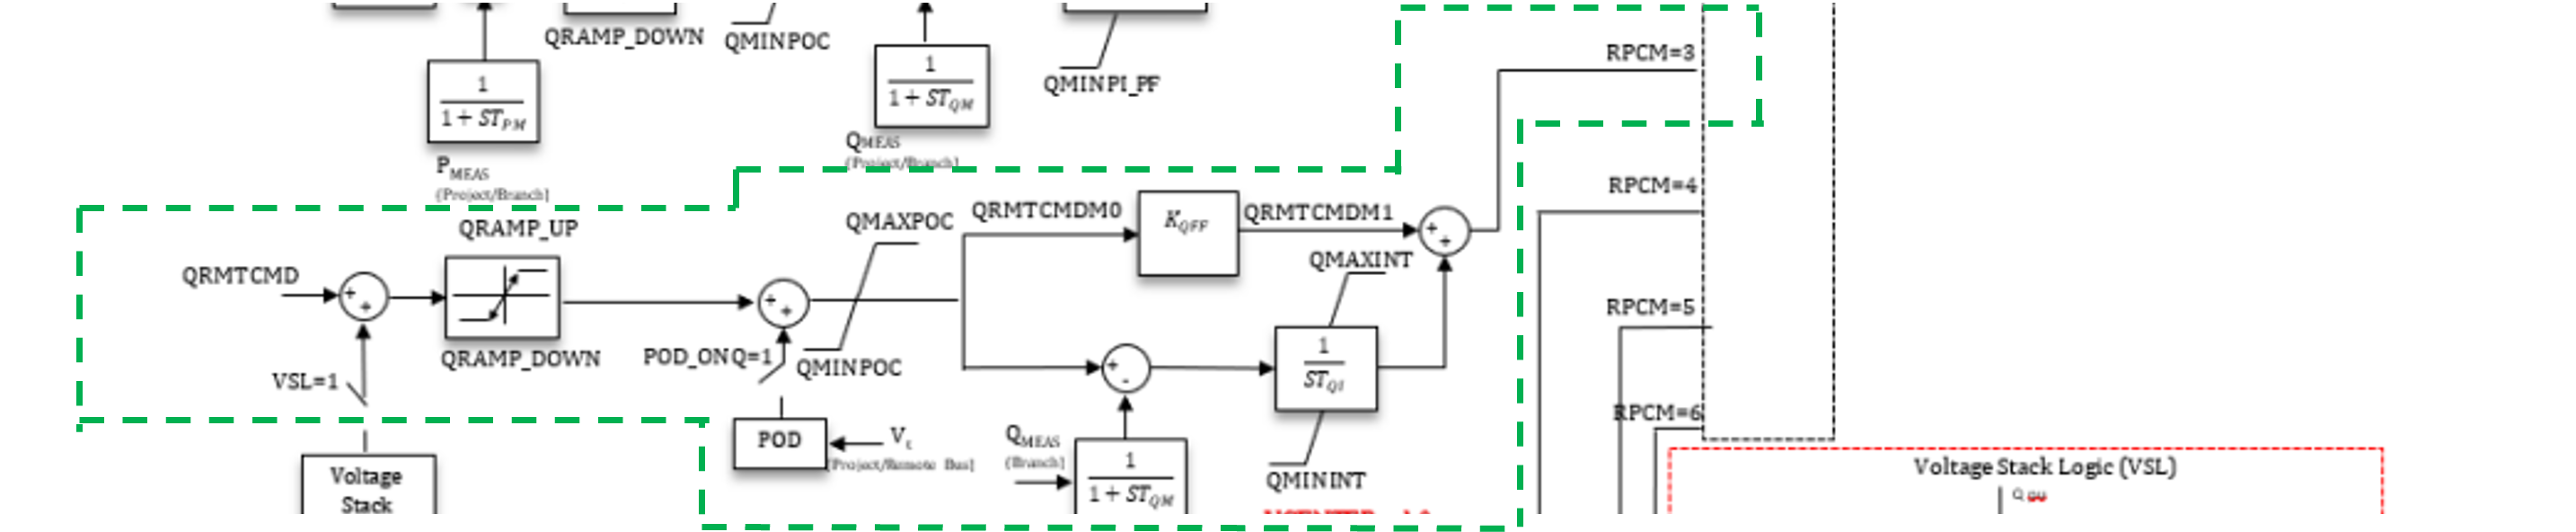
\includegraphics[width=0.6\textwidth]{report-assets/images/q-mode-block-diagram.png}
		\caption{Power factor control block diagram}
		\label{fig:q-block-diagram}
	\end{figure}
	
	
	\subsubsection{Power factor control}
	
	Power factor control is available in the PPC. This allows the PPC to target a constant power factor at the point of connection within the limits of the plant rating. The block diagram for the power factor control mode is shown in Figure \ref{fig:pf-block-diagram}.
	
	\begin{figure}[H]
		\centering
		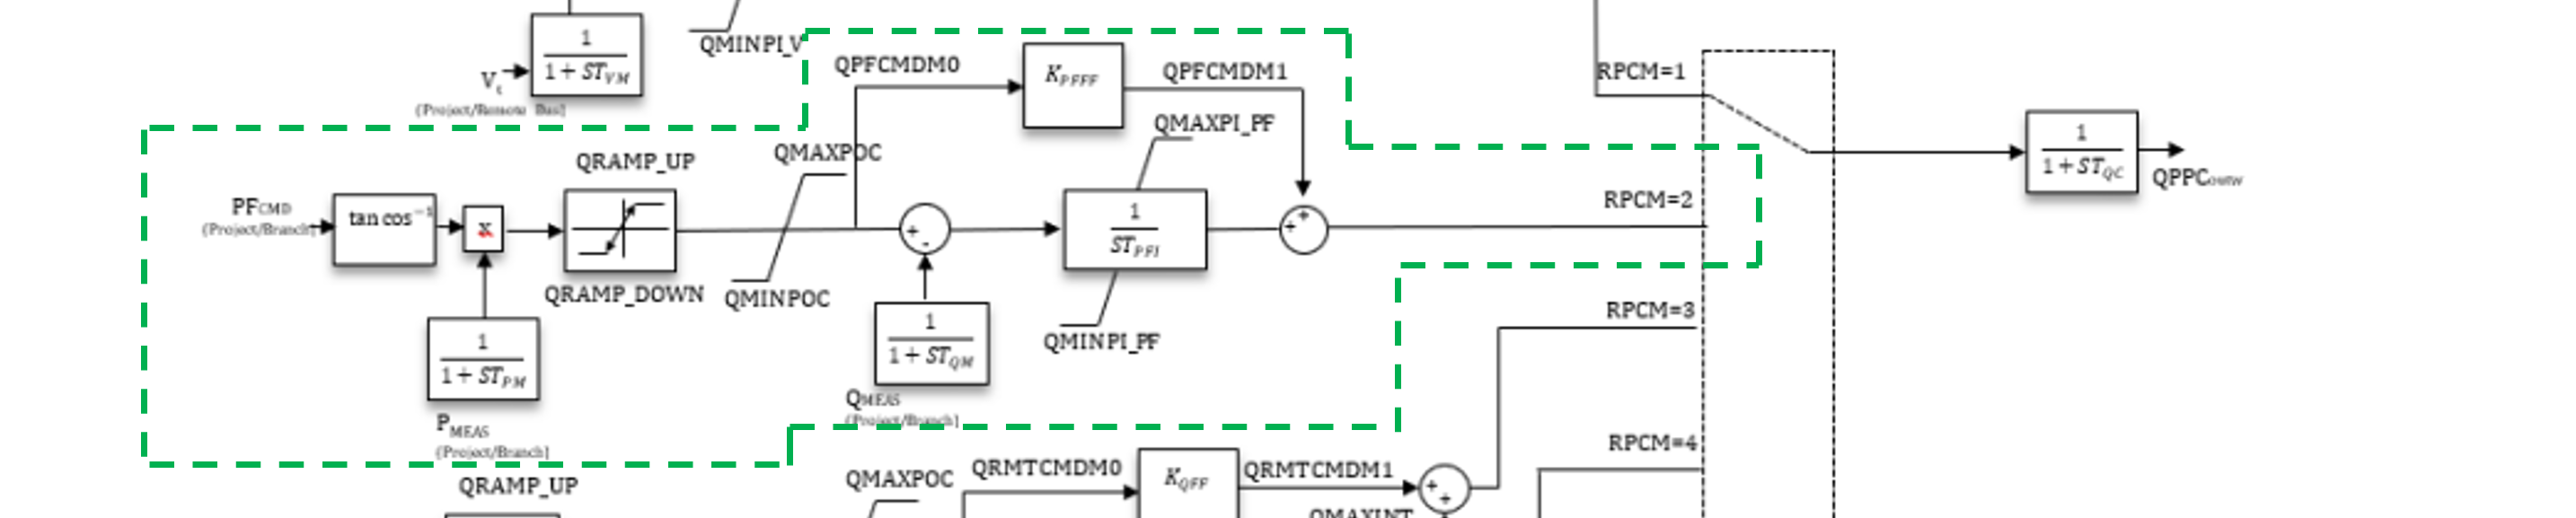
\includegraphics[width=0.6\textwidth]{report-assets/images/pf-mode-block-diagram.png}
		\caption{Power factor control block diagram}
		\label{fig:pf-block-diagram}
	\end{figure}

	\subsection{OLTC control}
	
	The 275/33/33 kV three-winding transformer is equipped with an on-load tap changer. The OLTC voltage set point is expected to be set to a fixed value of 1.0 pu, independent of the level of generation. The OLTC \ac{AVR} relay utilises a dead band ensuring that the target is achieved to within $\pm$ 0.015 pu. The transformer is set to operate with a time delay of 20 seconds and 7s mechanical operation time. If after a single tap change operation the voltage is still outside the deadband, another tap command will be expected after an additional 20 seconds. This time delay has been selected to ensure no unwanted interference between primary and secondary control loops while ensuring it is fast enough to ensure the generator maintains continuous uninterrupted operation for a variety of network disturbances.
	
	{
		\thicktablelines
		\begin{longtable}{|C{6cm}|C{4cm}|} 
			\caption{Grid transformer OLTC Details}
			\label{tab:main-transformer}
			\\	
			\toprule
			
			\rowcolor{tableheaderblue}
			\bfseries \color{white}Parameter & \bfseries \color{white}Value\\
			\endhead
			\bottomrule \endfoot
			\csvreader[
			separator=semicolon,
			late after line=\\\hline,
			late after last line=,
			before reading={\catcode`\#=12},
			after reading={\catcode`\#=6}]%
			{report-assets/main_transformer.csv}{1=\CSVParameter,2=\CSVValue}{\CSVParameter &\CSVValue}
			\\\hline
		\end{longtable}
	}

	
	OLTC control has been specified for the plant to tap the HV winding of the 3 winding grid transformer, while measuring one of the two medium voltage 33 kV plant buses. This control has been specified to accomplish the following objectives:
	
	\begin{itemize}
		\item Regulation of voltage to enable plant to meet its continuous uninterrupted operational requirements. 
		\item Regulation of voltage on both plant 33 kV buses without the need for two tap changers per transformer.
		\item Sufficient delay to avoid interference with faster acting plant control systems, such as the PPC response under voltage droop control.
	\end{itemize}
	
	\subsection{Inverter level control}
	\label{sec:inverter-level-control}
	SMA inverters are grid-forming and support inverter-level reactive and active power droop control, as well as inertia control. The default operating mode for the inverter is 22321 – P-Inertia and Q-Droop.
	
	\subsubsection{Reactive power control}
	
	The SMA inverters are grid-forming and capable of operating independently to regulate voltages at their terminals. Under normal operation the grid-forming inverters act as an inner loop control, regulating reactive power output based on a droop setting (of 0.1) independent of the PPC droop during dynamic disturbances. As the outer-loop is regulated by the PPC, the plant will always settle with regards to the PPC droop setting, but performance of the plant during disturbances or reference changes is dependent on this inner loop droop setting.
	
	\subsubsection{Fault ride through mode}
	
	The \ac{FRT} mode of the grid forming converters is defined by parameter GriForm.Frt.Mod (PSCAD: GriForm_Frt_Mod).The available modes are:
	
		\begin{itemize}
		\item Disabled (GRIFORM_FRT_MOD_DISABLE) 
		\item Full Virtual Impedance (GRIFORM_FRT_MOD_FULL_VI)
		\item k-factor Basic (GRIFORM_FRT_MOD_FULL_VI_K_FAC_BASIC)
		\item k-factor Advanced (GRIFORM_FRT_MOD_FULL_VI_K_FAC_ADVANCED).		
	\end{itemize}
	
	The selected operating mode is "k-factor advanced", which uses a virtual impedance to establish a k-factor characteristic to limit the current.  This helps shape the inverter's response during a fault by emulating an impedance (resistance + reactance) between the inverter voltage source and the grid.
	
	Unlike grid-following plant, the fault ride through mode of the SMA GFM converters does not have settable entry and exit thresholds. Transition into the "virtual impedance" mode is done based on detection of significant voltage changes at the inverter terminal, which are not configurable by default in the power system model. To prevent windup, the PPC will freeze operation when system voltages are outside of selected thresholds of 0.85 and 1.15 p.u, which means control is done at the inverter level under fault conditions. When in FRT, the active and reactive current contribution of the plant is similar to a strategy set by grid following converters. The configured settings have been set so that:
	
	\begin{itemize}
		\item The k-factor equivalent gain of the converters during FRT is 6, which implies a 6\% contribution per 1\% change in voltage measured at the inverter terminals.
		\item Negative sequence current gain of the converters has also been set to 6.
		\item Reactive current contribution is limited to a peak of 1.3 p.u. of the continuous current rating of the converters.
	\end{itemize} 
	
	During FRT, the converters will not actively control voltages, but will support voltages by provision of reactive current until a fault is cleared by protection. Plant response is not co-ordinated at the point of connection, but is dependant on converter terminal voltage during these events.

	\chapter{Reactive capability}
	The reactive capability curves for \ac{Heywood BESS} at 35°C, 40°C and 50°C are shown in Figures \ref{fig:pq-curve-35degC}, \ref{fig:pq-curve-40degC} and \ref{fig:pq-curve-50degC}. The automatic access standard has been shown as a dotted line, and is defined by the upper corner points $P_{max}$=285 MW, $Q_{max}$=112.575 MVAr, $P_{max}$=285 MW, $Q_{min}$=-112.575 MVAr, and the lower corner points $P_{min}$=-285 MW, $Q_{min}$=-112.575 MVAr, $P_{min}$=-285 MW, $Q_{max}$=112.575 MVAr.
	
	
	\begin{figure}[H]
		\centering
		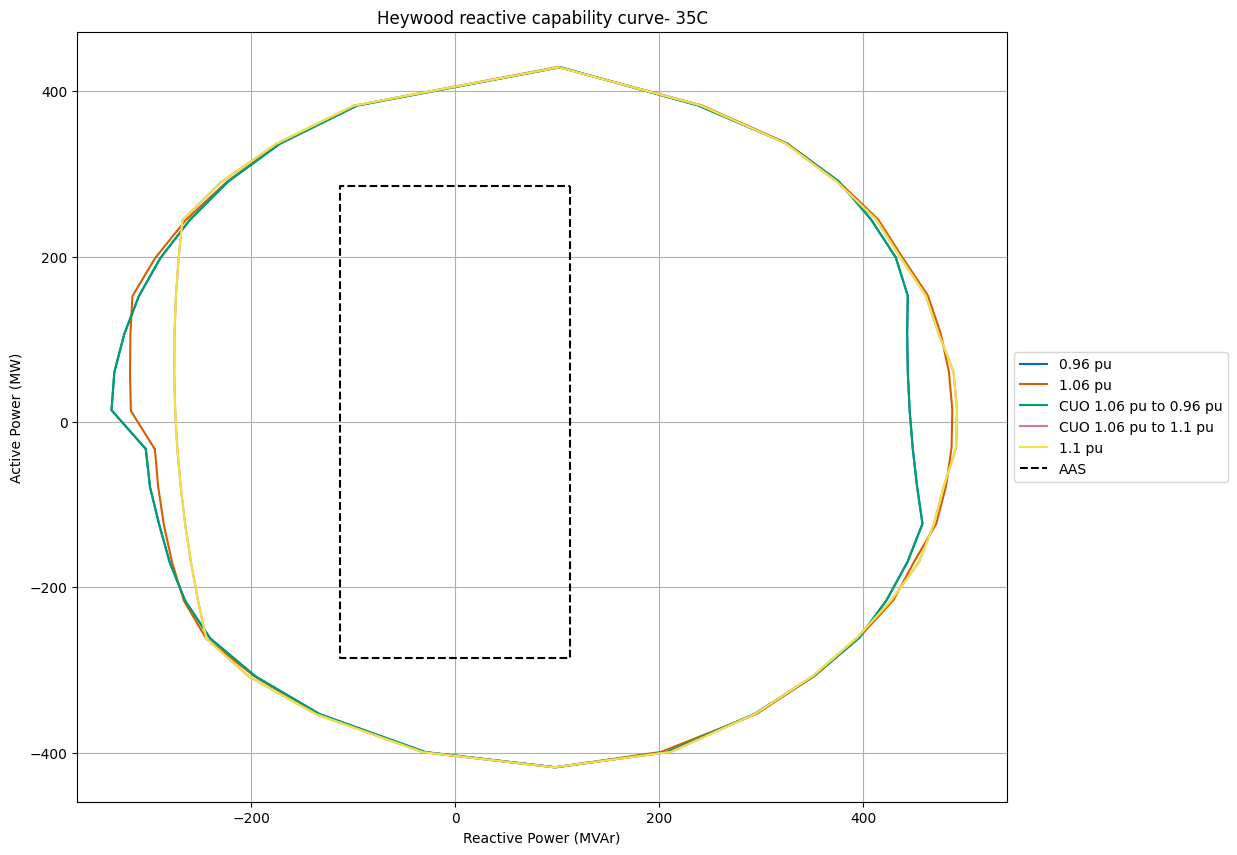
\includegraphics[width=0.8\textwidth]{\projectassetsdir/capability-curves/new_Heywood reactive capability curve- 35C.png}
		\caption{35°C Reactive capability curve for Heywood BESS}
		\label{fig:pq-curve-35degC}
	\end{figure}
	
	\begin{figure}[H]
		\centering
		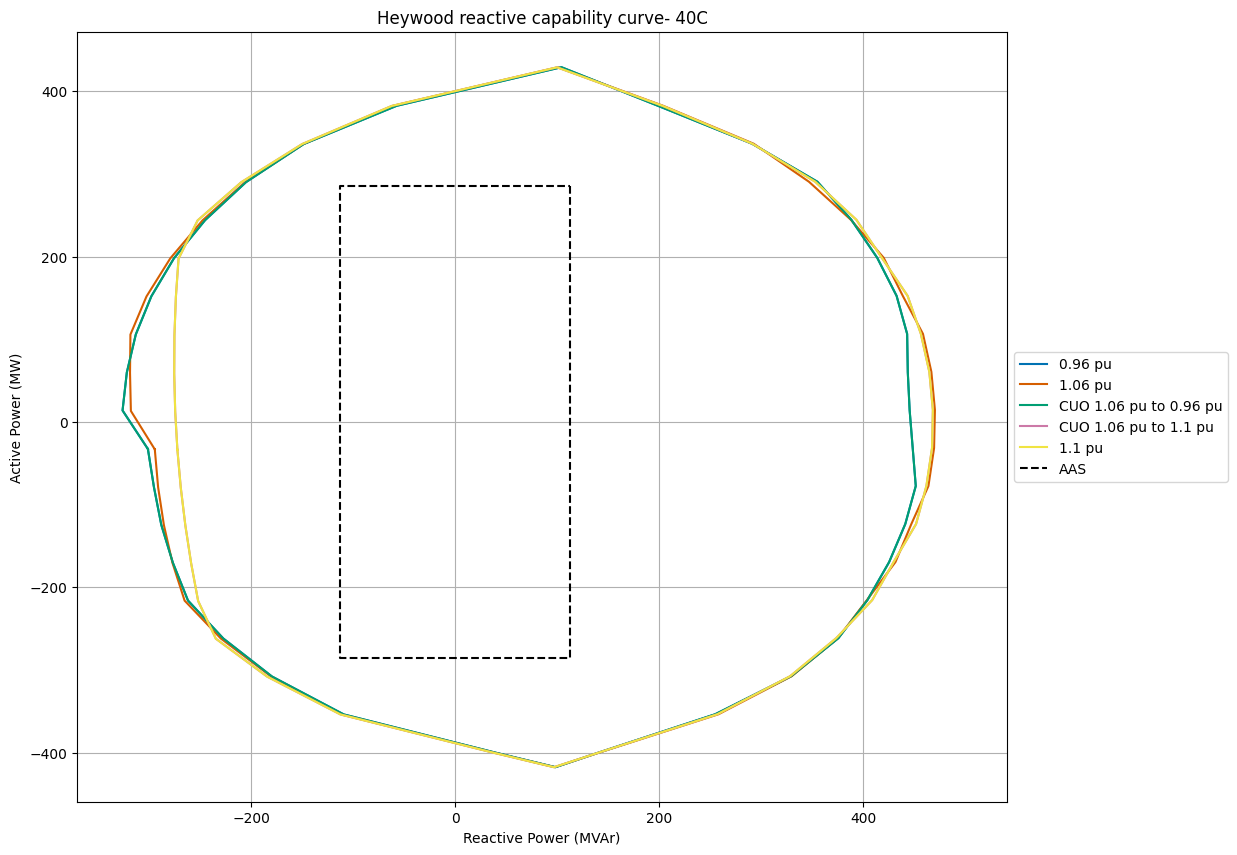
\includegraphics[width=0.8\textwidth]{\projectassetsdir/capability-curves/new_Heywood reactive capability curve- 40C.png}
		\caption{40°C Reactive capability curve for Heywood BESS}
		\label{fig:pq-curve-40degC}
	\end{figure}
	
	\begin{figure}[H]
		\centering
		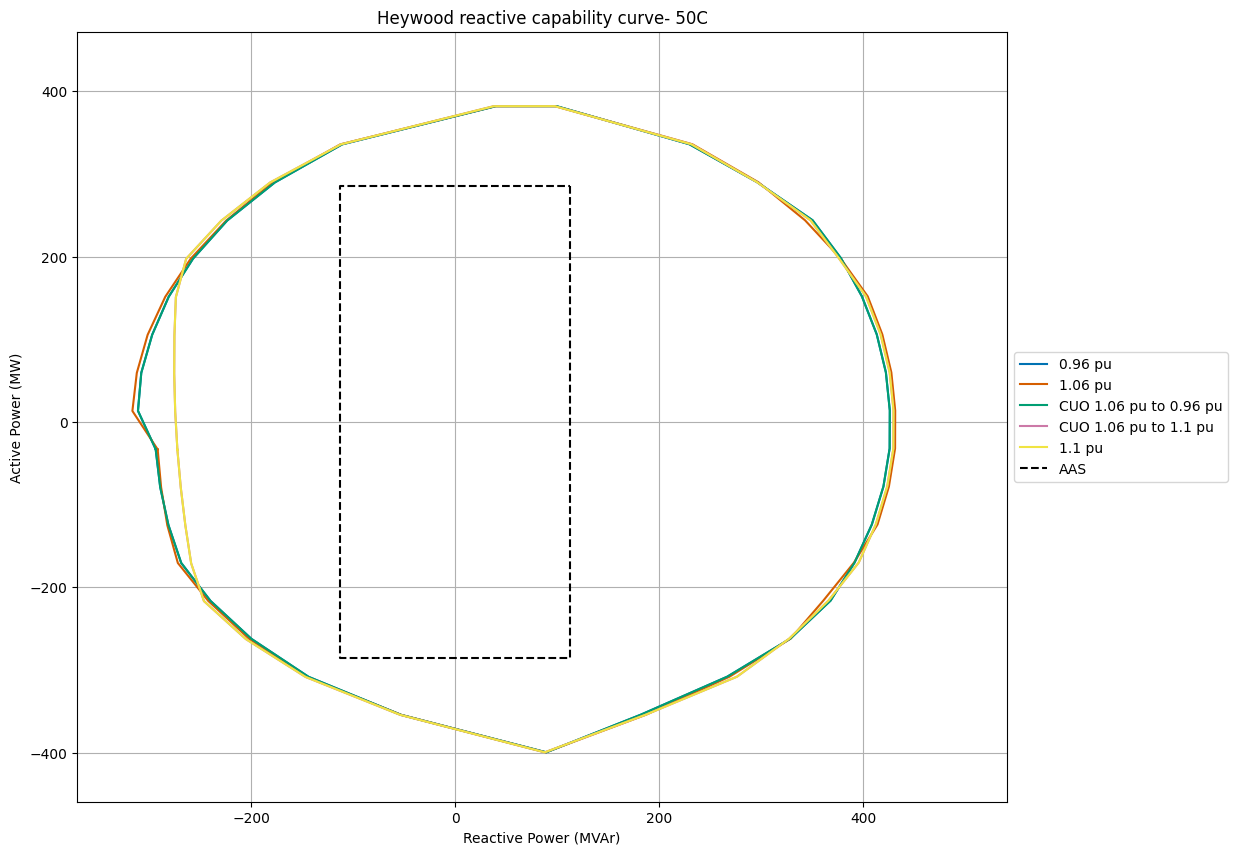
\includegraphics[width=0.8\textwidth]{\projectassetsdir/capability-curves/Heywood reactive capability curve- 50C.png}
		\caption{50°C Reactive capability curve for Heywood BESS}
		\label{fig:pq-curve-50degC}
	\end{figure}
	
	\chapter{Voltage protection}
	
	The converters are equipped with voltage protection, which have been set as per the maximum capability of the plant converters at their terminals. The voltage protection characteristic is shown in Figure \ref{fig:vprotection}.
	
	\begin{figure}[H]
		\centering
		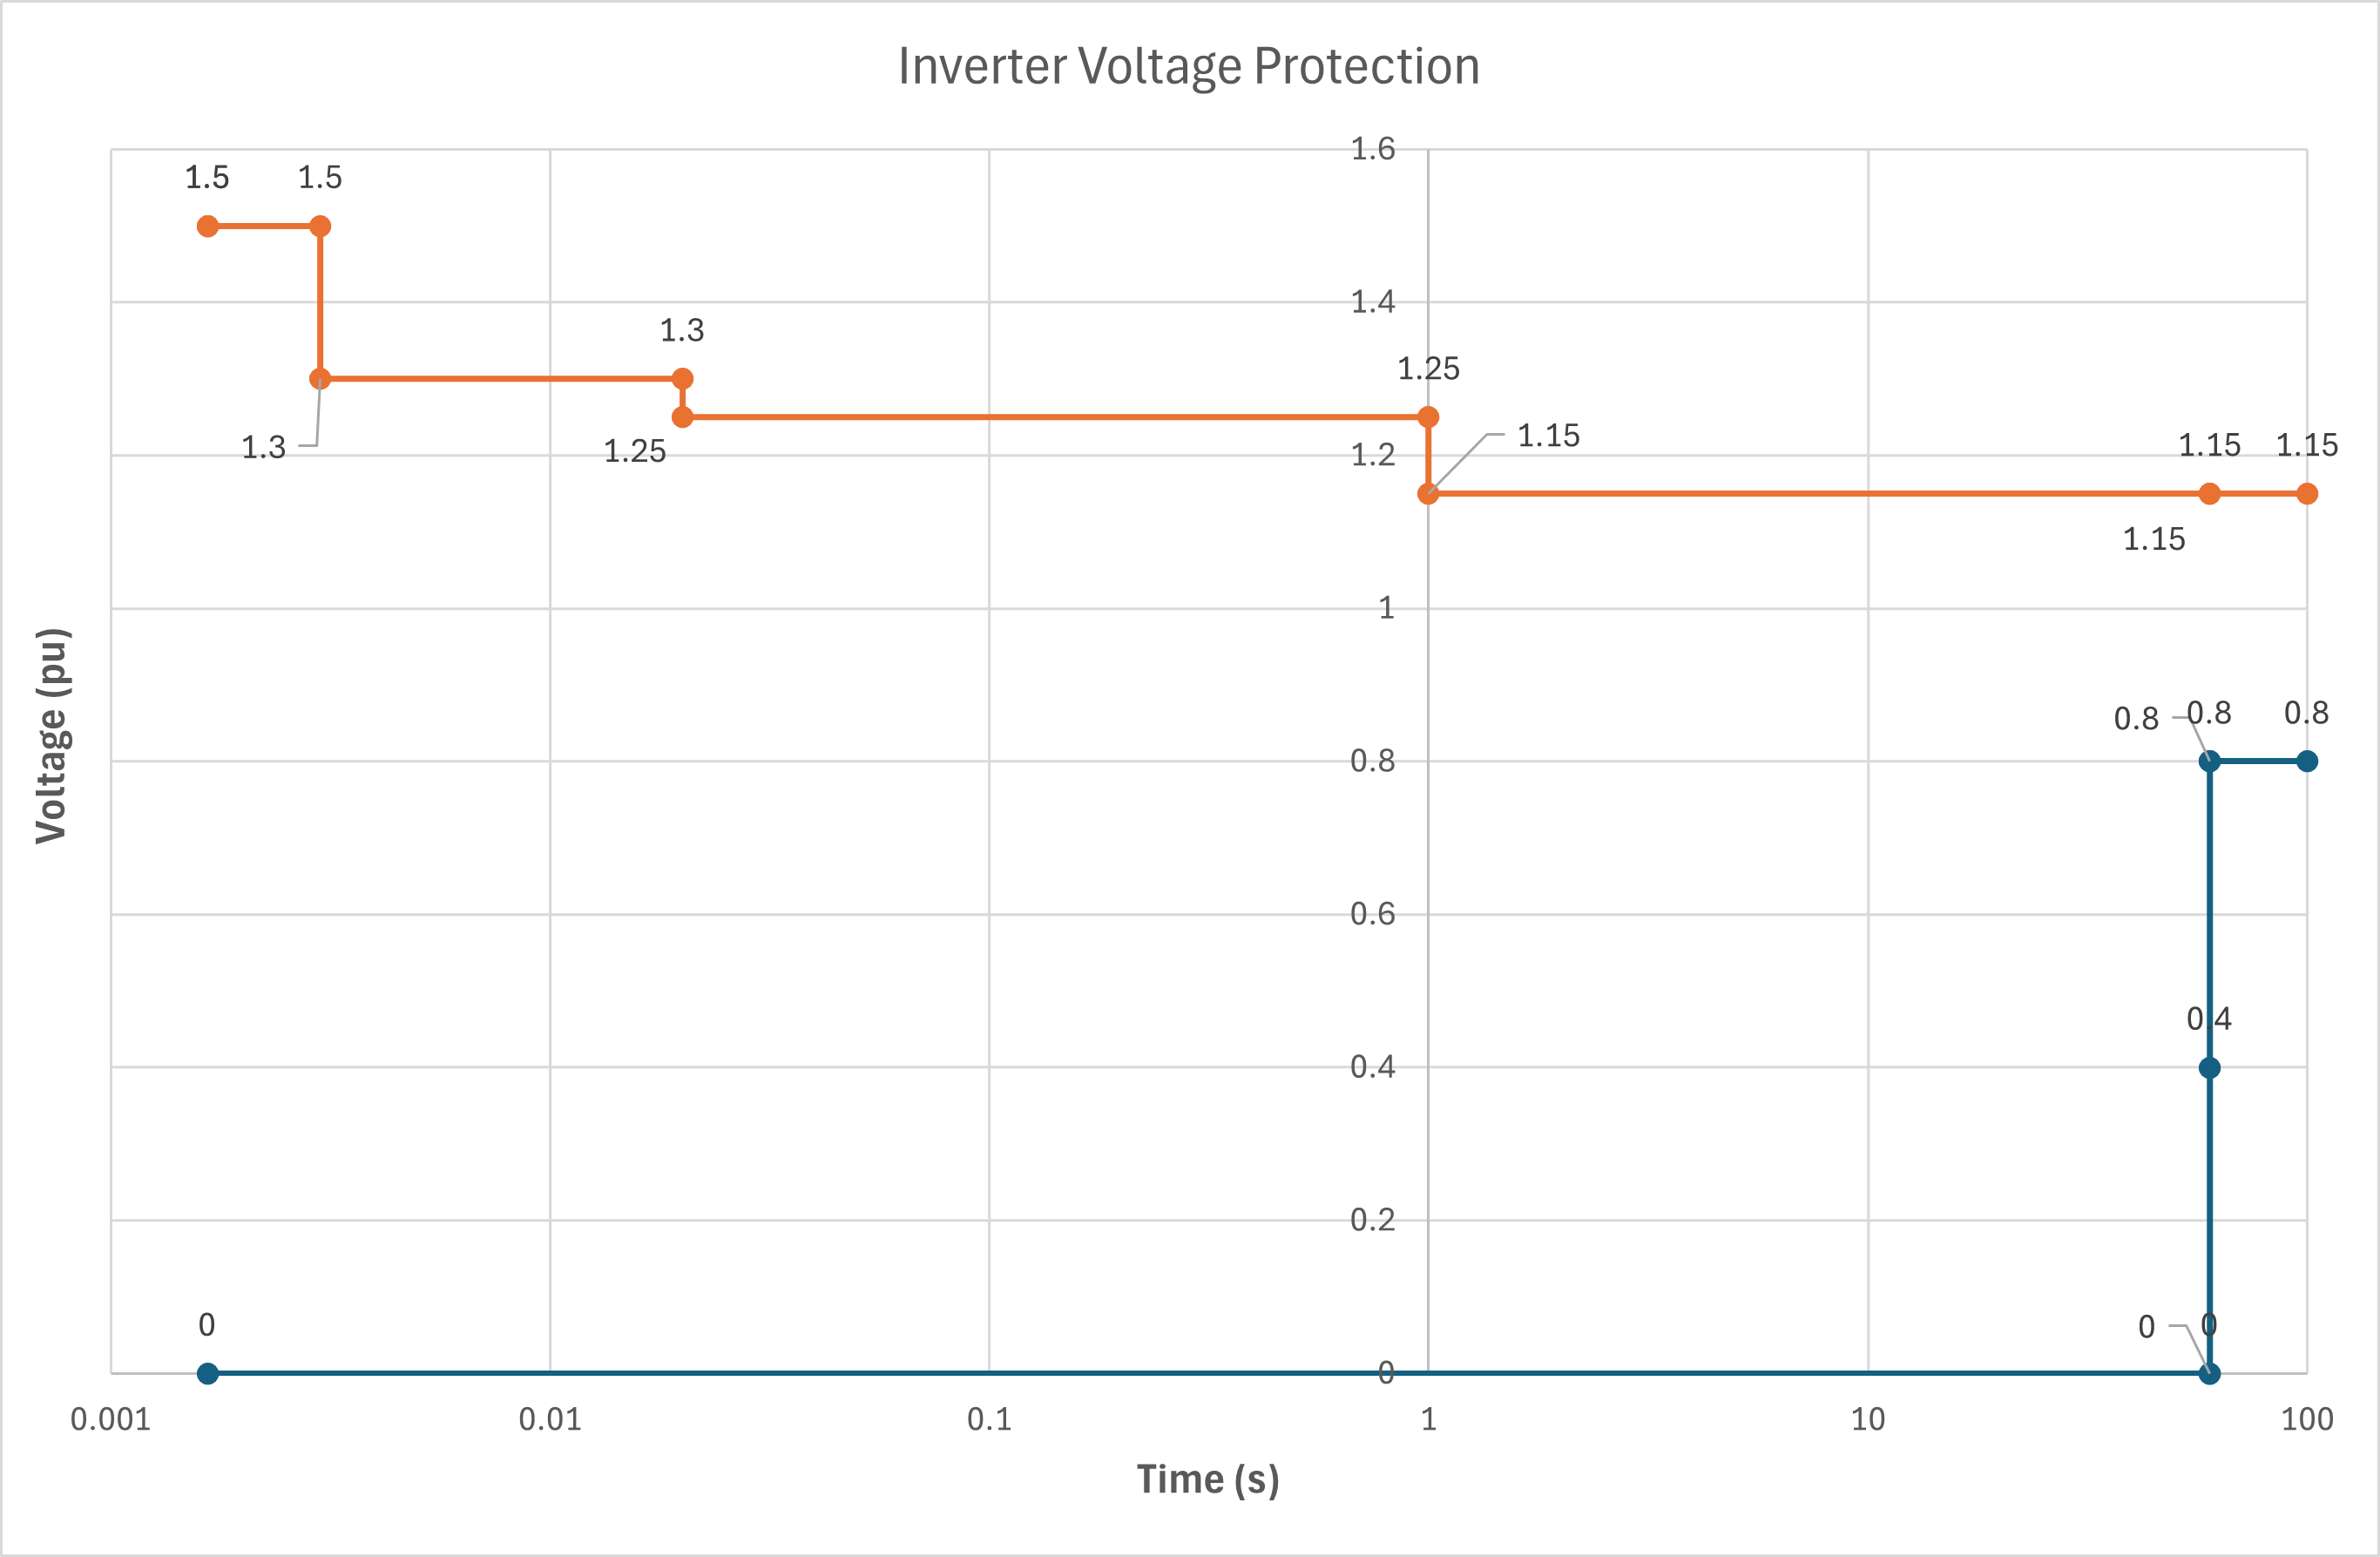
\includegraphics[width=0.6\textwidth]{report-assets/images/vprotection-new.png}
		\caption{Voltage protection characteristics}
		\label{fig:vprotection}
	\end{figure}
	
	\chapter{Control mode switching}
	
	Heywood BESS is capable of operating in three main reactive power control modes. Transfer between these modes is done by the modification of two parameters in the PPC.
	
	\begin{itemize}
		\item Reactive power control mode can be selected by changing the RPCM parameter to mode 3.
		\item Power factor control mode can be selected by changing the RPCM parameter to mode 2.
		\item Voltage droop mode can be selected by changing the RPCM parameter to mode 5.
		\item Reactive power and power factor control that \ac{VSL} is disabled. This is done by setting the parameter VSL to zero.
		\item Voltage droop control requires that voltage stack logic is enabled. This is done by setting the parameter VSL to one.
	\end{itemize}
	
	Transfer between voltage control modes can be done with the PPC online. The BESS \ac{EMS} is responsible for ensuring that switching between these modes, whether by a local operator or a remote party is bumpless - which is to say there will not be large changes in reactive power output when transitioning between reactive power modes. 
	
	\chapter{Control block diagrams and communications delays}
	
	Detailed control block diagrams for plant converters will be provided directly to AEMO by SMA and will not be displayed in this document due to confidentiality. 
	
	The block diagram of the PPC reactive power control modes has been extracted from the Fluence PPC manual and is shown in Figure \ref{fig:ppc-block-q-diagram}. Mode(s) 2, 3 and 5 are active for this plant.
	
	\begin{figure}[H]
		\centering
		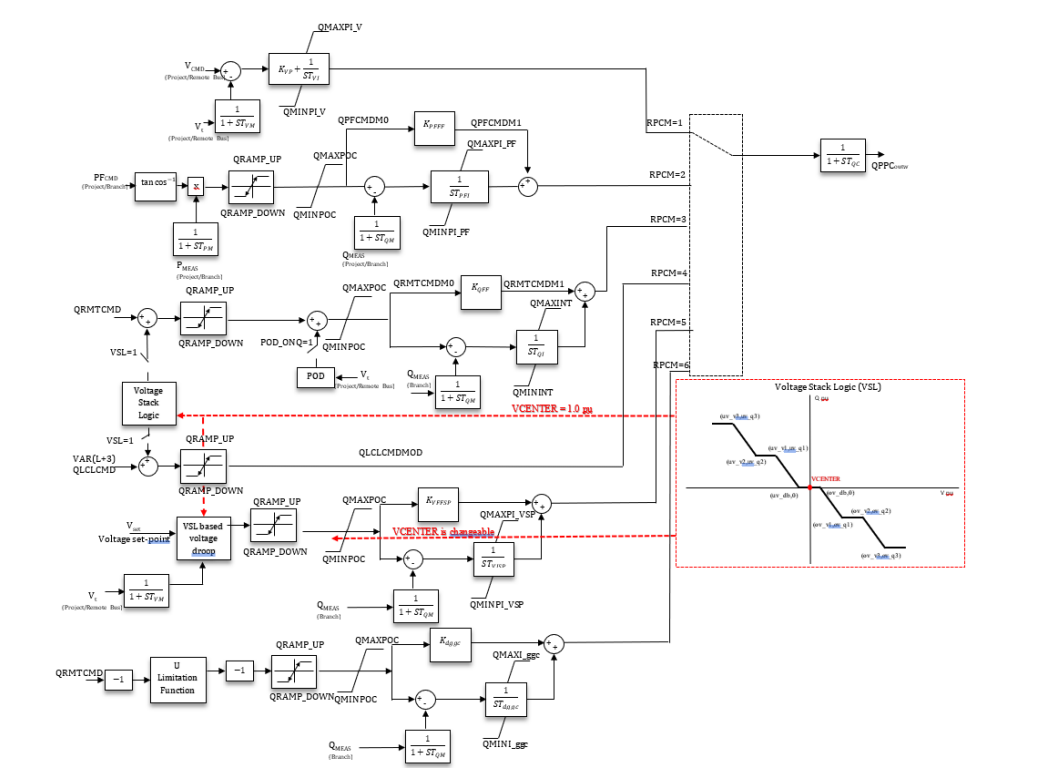
\includegraphics[width=0.6\textwidth]{report-assets/images/ppc-qmode-diagram.png}
		\caption{PPC reactive power control block diagram}
		\label{fig:ppc-block-q-diagram}
	\end{figure}
	
	The Fluence PPC has several inbuilt delays which are selected to represent the inherent delays in the measurement of inputs and output of plant setpoints. Key delays within the PPC applicable to the plant control are shown in Table \ref{tab:comms-delays}.
	
	{
		\thicktablelines
		\begin{longtable}{|C{8cm}|C{2cm}|} 
			\caption{Measurement and command delay times}
			\label{tab:comms-delays}
			\\	
			\toprule
			
			\rowcolor{tableheaderblue}
			\bfseries \color{white}Delay Variable & \bfseries \color{white}Value (s)\\
			\endhead
			\bottomrule \endfoot
			\csvreader[
			separator=semicolon,
			late after line=\\\hline,
			late after last line=,
			before reading={\catcode`\#=12},
			after reading={\catcode`\#=6}]%
			{report-assets/comms_delays.csv}{1=\CSVParameter,2=\CSVValue}{\CSVParameter &\CSVValue}
			\\\hline
		\end{longtable}
	}
	
	Measurement and command delay times have not been reduced below the default levels set in Fluence's PPC manual. The PPC freeze command delay has been increased from default level, as this modification was found to significantly improve performance following FRT exit, as this reduced PPC windup occurring while the plant responded to inverter level droop control set-points.


	\renewcommand\bibname{References}

\begin{thebibliography}{99}	
	\bibitem{mvps-sld}MVPS SLD\\
	(PSD1834-110-001-002.pdf)
	\bibitem{mvt-datasheet}Medium Voltage Transformer Datasheet\\
	(CG_D_00181175_03_General MVT Datasheet.pdf.pdf)
	\bibitem{main-tx-datasheet} Main Transformer Datasheet\\
	(Main Transformer Datasheet.pdf)
	\bibitem{substation-sld} Substation SLD\\
	(PSD1834-110-001-001.pdf)
	\bibitem{avr-manual}TAPCON 230 AVR manual\\
	(bal_3552133_02_001_1_en.pdf)
	\bibitem{oltc-switching} OLTC Switching Datasheet\\
	(VACUTAP®_VV®_Operating_Instructions.pdf)
	\bibitem{harmonic-assessment} Harmonic Emmissions Report\\
	(PSD1834-100-100---Harmonic-Emissions-Assessment-and-Filter-Design-Rev-B.pdf)
	\bibitem{scada-philo} SCADA Control Philosophy\\
	(PSD1834-200-009---SCADA-CONTROL-PHILOSOPHY-Rev.3.pdf)
	\bibitem{aemo-io} AEMO IO Schedule\\
	(PSD1834-200-005-AEMO IO SCHEDULE-REV-04.pdf)
	\bibitem{comms-arch} Communication Architecture\\
	(PSD1834-210-003-001---COMMUNICATION-ARCHITECTURE-Rev.1.pdf)
	\bibitem{scada-spec} SCADA Functional Specification\\
	(PSD1834-200-001 - SCADA SYSTEM FUNCTIONAL DESIGN SPECIFICATION Rev.4.pdf)
	\bibitem{protection-settings-report} Protection Settings Report\\
	(PSD1834-100-007---CGBESS-Protection-Setting-Report---REV-C.pdf)



\end{thebibliography}
	\chapter*{Acronyms}
\begin{acronym}%[JSONP]\itemsep0pt
	\acro{AAS}{Automatic Access Standard}
	\acro{AEMO}{Australian Energy Market Operator}
	\acro{VSL}{Voltage Stackable Logic}
	\acro{AGC}{Automatic Generation Control}
	\acro{AVR}{Automatic Voltage Regulator}
	\acro{BESS}{Battery Energy Storage System}
	\acro{BOP}{Balance Of Plant}
	\acro{CGBESS}{Clements Gap BESS}
	\acro{Heywood BESS}{Heywood Battery Energy Storage System}	
	\acro{CSR}{Connection Studies Report}
	\acro{CT}{Current Transformer}
	\acro{CUO}{Continuous Uninterrupted Operation}
	\acro{HV}{High Voltage}
	\acro{DMAT}{Dynamic Model Acceptance Test}
	\acro{DYR}{PSSE Dynamics Data File}
	\acro{EMT}{Electromagnetic Transients}
	\acro{FIA}{Full Impact Assessment}
	\acro{FRT}{Fault Ride-Through}
	\acro{GPS}{Generator Performance Standards}
	\acro{HVRT}{High Voltage Ride-Through}
	\acro{LV}{Low Voltage}
	\acro{LVRT}{Low Voltage Ride-Through}
	\acro{MV}{Medium Voltage}
	\acro{NEM}{National Electricity Market}
	\acro{NSP}{Network Service Provider}
	\acro{OEM}{Original Equipment Manufacturer}
	\acro{OFRT}{Over-Frequency Ride-Through}
	\acro{OLTC}{On-Load Tap Changer}
	\acro{OPDMS}{Operations and Planning Data Management System}
	\acro{OVRT}{Over-Voltage Ride-Through}
	\acro{PLL}{Phase-Locked Loop}
	\acro{PLR}{Partial Load Rejection}
	\acro{PPC}{Power Plant Controller}
	\acro{PPM}{Power Plant Manager}
	\acro{RoCoF}{Rate of Change of Frequency}
	\acro{RMS}{Root Mean Square}
	\acro{RMU}{Ring Main Unit}
	\acro{RUG}{Releasable User Guide}
	\acro{S5251}{Reactive Power Capability}
	\acro{S5254}{Generating System Response to Voltage Disturbances}
	\acro{SCR}{Short Circuit Ratio}
	\acro{SMIB}{Single Machine, Infinite Bus}
	\acro{SLD}{Single Line Diagram}
	\acro{TOV}{Temporary Over-Voltage}
	\acro{UFRT}{Under-Frequency Ride-Through}
	\acro{UVRT}{Under-Voltage Ride-Through}
	\acro{VCS}{Voltage Control Strategy}
	\acro{WAN}{Wide Area Network}
	\acro{WF}{Wind Farm}
	\acro{VOIP}{Voice Over Internet Protocol}
	\acro{VRR}{Voltage Regulation Relay}
	\acro{VT}{Voltage Transformer}
\end{acronym}
	
	
	\makebackpage
	
	
	
	
	
\end{document}